% Figure 3: author-confirmed 144-paper corpus (69+42+33).
% Author-confirmed exclusions: 62+49+44+27=182; 326-182=144.
% Screening and eligibility arithmetic reconciled on 2 October 2026.
% Rebuild all figures from the project root: bash tkz/build.sh
\documentclass[tikz,border=0pt,class=IEEEtran]{standalone}
\usepackage{amsmath,amssymb,amsfonts}
\usepackage{xcolor}
\usetikzlibrary{positioning,arrows.meta,calc,backgrounds}

% Match the manuscript's IEEE Access text and math font settings.
\renewcommand{\textbf}[1]{{\fontseries{b}\selectfont #1}}
\renewcommand{\textit}[1]{{\itshape #1}}
\makeatletter
\AtBeginDocument{%
  \fontencoding{T1}\rmfamily\fontseries{m}\fontsize{10}{12}\selectfont
  \gdef\operator@encoding{T1}%
  \gdef\encodingdefault{T1}}
\makeatother

% ---- shared palette for review figures ----
\definecolor{cVLA}{HTML}{34618E}   % VLA lane / policy blue
\definecolor{cWM}{HTML}{9E4A3F}    % world-model lane
\definecolor{cGood}{HTML}{3A7D44}  % verified green
\definecolor{cWarn}{HTML}{B07A2A}  % caution amber
\definecolor{cPale}{HTML}{F2F0EA}  % pale panel fill
\tikzset{
  fnode/.style={draw=black!55, fill=white, rounded corners=1.5pt,
                inner sep=2.5pt, align=center, font=\scriptsize},
  flane/.style={draw=none, rounded corners=2pt, inner sep=3pt,
                align=center, font=\scriptsize\bfseries, text=white},
  farr/.style={-{Stealth[length=2mm]}, thick, black!60},
}

\begin{document}
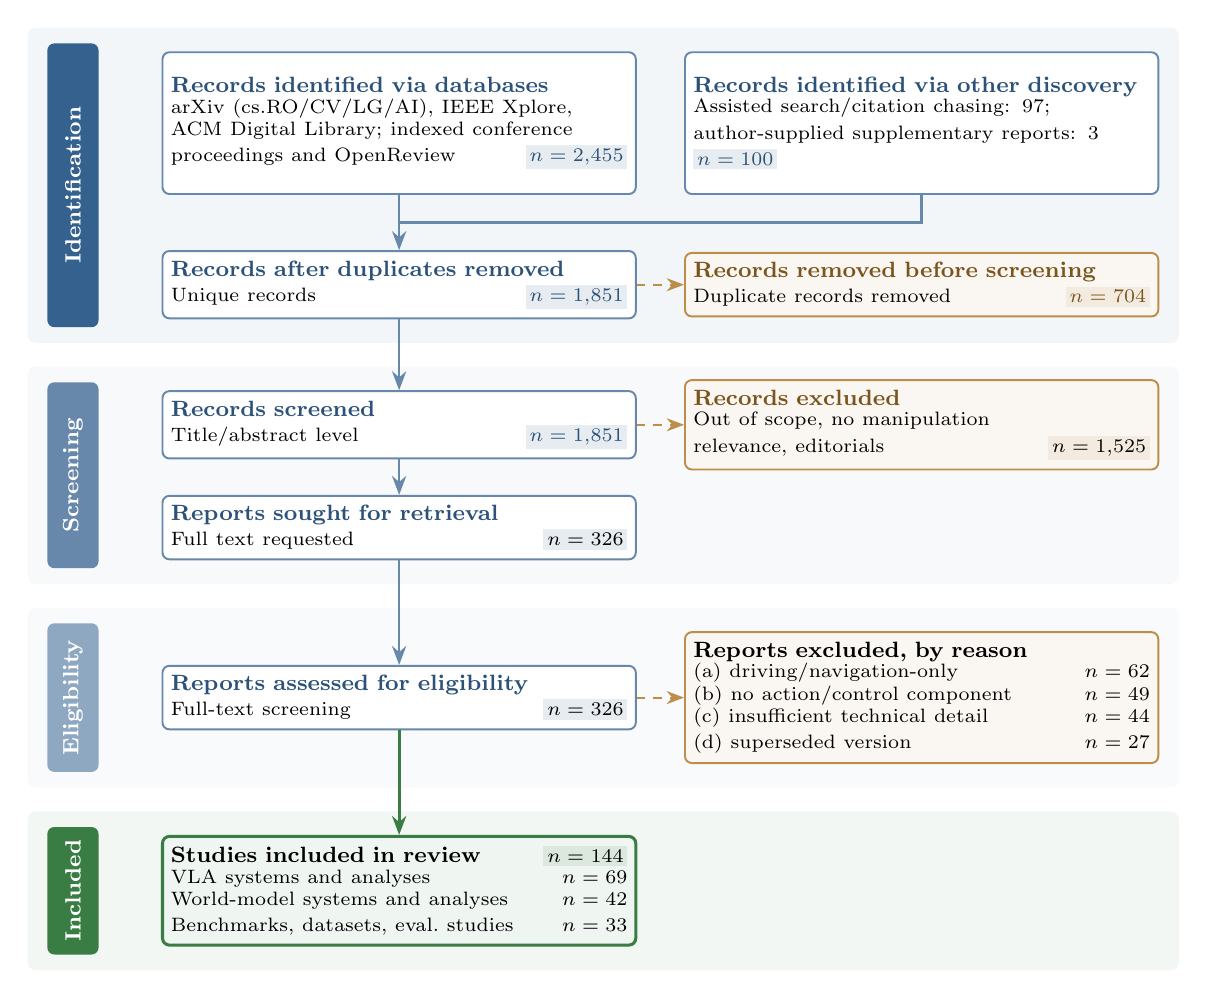
\begin{tikzpicture}[
  font=\footnotesize,
  % --- layout constants -------------------------------------------------
  boxw/.store in=\boxw,  boxw=58mm,     % text width of every box
  colgap/.store in=\colgap, colgap=6mm, % horizontal gap between columns
  rowgap/.store in=\rowgap, rowgap=4.5mm,% vertical gap inside a stage
  stagegap/.store in=\stagegap, stagegap=9mm, % vertical gap between stages
  % --- box styles ---------------------------------------------------------
  box/.style={rounded corners=2.5pt, align=left, inner xsep=3pt, inner ysep=3.5pt,
              text width=\boxw},
  pbox/.style={box, draw=cVLA!75, line width=0.7pt, fill=white},
  exbox/.style={box, draw=cWarn!85, line width=0.7pt, fill=cWarn!6},
  incbox/.style={box, draw=cGood, line width=1.1pt, fill=cGood!8},
  % --- arrows ---------------------------------------------------------------
  arr/.style={-{Stealth[length=2.4mm]}, line width=0.9pt, cVLA!75},
  jline/.style={line width=0.9pt, cVLA!75},
  exarr/.style={-{Stealth[length=2.2mm]}, line width=0.8pt, cWarn!85, dashed},
]
% ---- shorthand: box content = [title | details] with a right-aligned badge
\newcommand{\ptitle}[1]{{\color{cVLA!85!black}\bfseries #1}}
\newcommand{\extitle}[1]{{\color{cWarn!70!black}\bfseries #1}}
\newcommand{\prBadge}[3]{{\scriptsize\setlength{\fboxsep}{1.4pt}%
  \colorbox{#1}{\textcolor{#2}{\bfseries #3}}}}
\newcommand{\nbadge}[1]{\prBadge{cVLA!12}{cVLA!85!black}{#1}}
\newcommand{\exbadge}[1]{\prBadge{cWarn!15}{cWarn!70!black}{#1}}
% \prBox{title}{details}{badge}: full-width title line, details in
% \scriptsize, count badge right-aligned on the last details line
\newcommand{\prBox}[3]{#1\\[-0.5pt]{\scriptsize #2\hfill #3}}
% ======================= main (centre) column ==============================
\node[pbox, minimum height=18mm] (dbs)
  {\prBox{\ptitle{Records identified via databases}}
  {arXiv (cs.RO/CV/LG/AI), IEEE Xplore,\\
   ACM Digital Library; indexed conference\\
   proceedings and OpenReview}{\nbadge{$n=2{,}455$}}};
\node[pbox, minimum height=18mm, right=\colgap of dbs] (other)
  {\prBox{\ptitle{Records identified via other discovery}}
  {Assisted search/citation chasing: 97;\\
   author-supplied supplementary reports: 3}{\nbadge{$n=100$}}};
\node[pbox, below=7mm of dbs] (dedup)
  {\prBox{\ptitle{Records after duplicates removed}}
  {Unique records}{\nbadge{$n=1{,}851$}}};
\node[pbox, below=\stagegap of dedup] (screen) {\prBox{\ptitle{Records screened}}
  {Title/abstract level}{\nbadge{$n=1{,}851$}}};
\node[pbox, below=\rowgap of screen] (retr) {\prBox{\ptitle{Reports sought for retrieval}}
  {Full text requested}{\prBadge{cVLA!12}{black}{$n=326$}}};
% ======================= exclusion (right) column ===========================
% each side box is vertically centred on its main-column row
\node[exbox, right=\colgap of dedup] (exdedup) {\prBox{\extitle{Records removed before screening}}
  {Duplicate records removed}{\exbadge{$n=704$}}};
\node[exbox, right=\colgap of screen] (exscreen) {\prBox{\extitle{Records excluded}}
  {Out of scope, no manipulation\\ relevance, editorials}{\prBadge{cWarn!15}{black}{$n=1{,}525$}}};
% Keep the reasons box at the existing stage top and center the assessment box beside it.
\node[exbox, anchor=north west] at ([xshift=\colgap,yshift=-\stagegap]retr.south east) (exelig)
{\textcolor{black}{\bfseries Reports excluded, by reason}\\[-0.5pt]
{\scriptsize
 (a) driving/navigation-only \hfill $n=62$\\
 (b) no action/control component \hfill $n=49$\\
 (c) insufficient technical detail \hfill \textcolor{black}{$n=44$}\\
 (d) superseded version \hfill $n=27$}};
\node[pbox] at (retr.center |- exelig.center) (elig)
  {\prBox{\ptitle{Reports assessed for eligibility}}
  {\textcolor{black}{Full-text screening}}{\prBadge{cVLA!12}{black}{$n=326$}}};
% ======================= included ==========================================
% placed below the taller of {elig, exelig}, centred on the main column
\node[incbox, anchor=north] at ([yshift=-\stagegap]elig.south |- exelig.south) (incl)
{{\color{black}\bfseries Studies included in review}\hfill
 \prBadge{cGood!18}{black}{$n=144$}\\[-0.5pt]
 {\scriptsize
  VLA systems and analyses \hfill \textcolor{black}{$n=69$}\\
  World-model systems and analyses \hfill \textcolor{black}{$n=42$}\\
  Benchmarks, datasets, eval.\ studies \hfill \textcolor{black}{$n=33$}}};
% ======================= stage tabs + bands ================================
% Tab and band are drawn from the *same* vertical extent (top node .north to
% bottom node .south), so they are aligned by construction.
\coordinate (tabL) at ([xshift=-14.5mm]dbs.west);
\coordinate (tabR) at ([xshift=-8mm]dbs.west);
\newcommand{\prStage}[5]{% {colour}{top node}{bottom node}{label}{band tint}
  \begin{scope}[on background layer]
    \fill[#5, rounded corners=3pt]
      ([xshift=-2.5mm, yshift=3mm]tabL |- #2.north)
      rectangle ([xshift=2.5mm, yshift=-3mm]other.east |- #3.south);
  \end{scope}
  \fill[#1, rounded corners=2.5pt]
    ([yshift=1mm]tabL |- #2.north) rectangle ([yshift=-1mm]tabR |- #3.south);
  \node[rotate=90, font=\footnotesize\bfseries, text=white, inner sep=0pt]
    at ($(tabL |- #2.north)!0.5!(tabR |- #3.south)$) {#4};
}
\prStage{cVLA}{dbs}{dedup}{Identification}{cVLA!6}
\prStage{cVLA!75}{screen}{retr}{Screening}{cVLA!4}
\prStage{cVLA!55}{exelig}{exelig}{Eligibility}{cVLA!3}
\prStage{cGood}{incl}{incl}{Included}{cGood!6}
% ======================= arrows ============================================
\coordinate (merge) at ($(dbs.south)!0.5!(dedup.north)$);
\draw[jline] (dbs.south) -- (merge);
\draw[jline] (other.south) |- (merge);
\draw[arr] (merge) -- (dedup.north);
\draw[arr]  (dedup)  -- (screen);
\draw[arr]  (screen) -- (retr);
\draw[arr]  (retr)   -- (elig);
\draw[arr, cGood, line width=1.1pt] (elig) -- (incl);
\draw[exarr] (dedup)  -- (exdedup);
\draw[exarr] (screen) -- (exscreen);
\draw[exarr] (elig.east) -- (elig.east -| exelig.west);
\end{tikzpicture}
\end{document}
